\chapter{降噪扩散模型生成中国画}

\section{模型概述}
降噪扩散模型,
也称为扩散模型,
在训练时分为添加噪声和去除噪声两部分,
首先,逐渐将随机噪声添加至图像,且对添加的噪声进行记录,最终获得均匀的噪声图像。
之后,对该噪声图像进行逐渐去噪,期望最终获得原始图像。
训练完成后,可以将任意的随机噪声,转化为与训练集中图像类似的图像。
算法{\ref{alg:diffusion_training}}为扩散模型训练算法,
算法{\ref{alg:diffusion_sampling}}为扩散模型采样算法。
% \begin{algorithm}[ht]
%     \caption{扩散模型训练算法}\label{alg:diffusion_training}
%     \begin{algorithmic}[1]
%         \REPEAT
%         \STATE{$\bm{x}_{0} \sim q(\bm{x}_{0})$}
%         \STATE{$t\sim \mbox{Uniform}(\{1,\ldots,T\})$}
%         \STATE{$\bm{\epsilon} \sim  \mathcal{N}(\bm{0},\bm{I})$}
%         \STATE{关于参数{$\theta$}进行梯度下降,梯度为{$\nabla_{\theta}{\Vert \bm{\epsilon} -\bm{\epsilon}_{\theta}(\sqrt{\bar{\alpha}_{t}}\bm{x}_{0}+\sqrt{1-\bar{\alpha}_{t}}\bm{\epsilon},t) \Vert}^{2}$}}
%         \UNTIL{收敛}
%     \end{algorithmic}
% \end{algorithm}
\begin{algorithm}[ht]
    \caption{扩散模型训练算法}\label{alg:diffusion_training}
    \begin{algorithmic}[1]
        \REPEAT
        \STATE{$\bm{x}_{0} \sim q(\bm{x}_{0})$}
        \STATE{$t\sim \mbox{Uniform}(\{1,\ldots,T\})$}
        \STATE{$\bm{\epsilon} \sim  \mathcal{N}(\bm{0},\bm{I})$}
        \STATE{关于参数{$\theta$}进行梯度下降,梯度为{$\nabla_{\theta}{\Vert \bm{\epsilon} -\bm{\epsilon}_{\theta}(\bm{x}_{t},t) \Vert}^{2}$}}
        \UNTIL{收敛}
    \end{algorithmic}
\end{algorithm}
\begin{algorithm}[ht]
    \caption{扩散模型采样算法}\label{alg:diffusion_sampling}
    \begin{algorithmic}[1]
        \STATE{$\bm{x}_{T}\sim \mathcal{N}(\bm{0},\bm{I})$}
        \FOR{$t=T,\ldots,1$}
        \STATE{$\bm{z}\sim \mathcal{N}(\bm{0},\bm{I})$}  if {$t>1$}, else {$\bm{z}=\bm{0}$}
        \STATE{$\bm{x}_{t-1}=\frac{1}{\sqrt{\alpha_{t}}}\left( \bm{x}_{t} - \frac{1-\alpha_{t}}{\sqrt{1-\bar{\alpha}_{t}}}\bm{\epsilon}_{\theta}(\bm{x}_{t},t) \right)+ \sigma_{q}(t)\bm{z}$}
        \ENDFOR
        \RETURN{{$\bm{x}_{0}$}}
    \end{algorithmic}
\end{algorithm}

扩散模型使用U型网络,U型网络的输入和输出维度相同。 
U型网络中,使用了上采样和下采样、残差连接、正弦位置嵌入以及注意力模块,
在注意力层前进行了组规范。

\section{数据集}
原始完整数据集{\cite{xue2020endtoend}}为从如下博物馆获取的高质量传统中国画:
\begin{itemize}
    \item 普林斯顿大学艺术博物馆362张;
    \item 哈佛大学艺术博物馆101张;
    \item 纽约大都会博物馆428张;
    \item 史密森尼弗里尔艺术画廊1301张。
\end{itemize}

共2194张高质量传统中国画,裁剪后大小均为{$512 \times 512$},
图{\ref{fig:complete_dataset_samples}}为完整数据集中国画采样。

在去除边缘留白较大的图像以及颜色过深的图像后,
对原始数据集根据颜色深浅进行分类,
得到包含1159张中国画的浅色中国画数据集,
以及包含792张中国画的深色中国画数据集。
图{\ref{fig:white_dataset_samples}}为浅色中国画数据集采样。
图{\ref{fig:yellow_dataset_samples}}为深色中国画数据集采样。
\begin{figure}[ht]
    \centering
    \subfigure{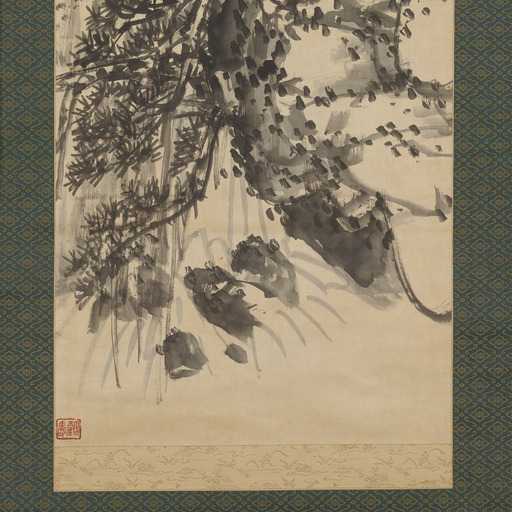
\includegraphics[width=0.2\textwidth, frame]{figures/diffusion/dataset_complete/Painting (1).jpg}}
    \subfigure{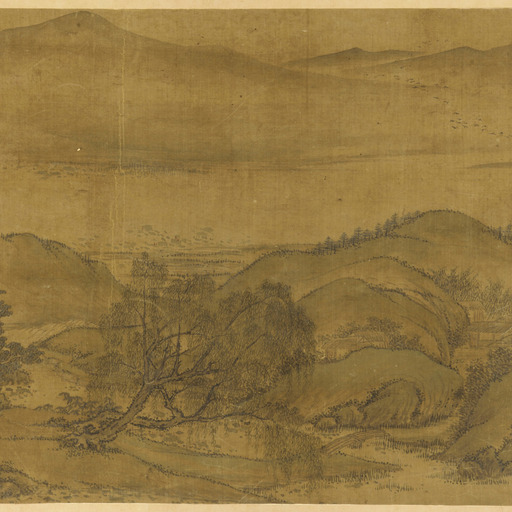
\includegraphics[width=0.2\textwidth, frame]{figures/diffusion/dataset_complete/Painting (2).jpg}}
    \subfigure{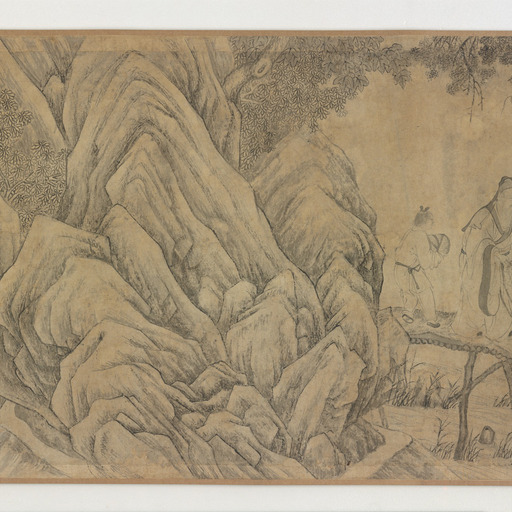
\includegraphics[width=0.2\textwidth, frame]{figures/diffusion/dataset_complete/Painting (3).jpg}}
    \subfigure{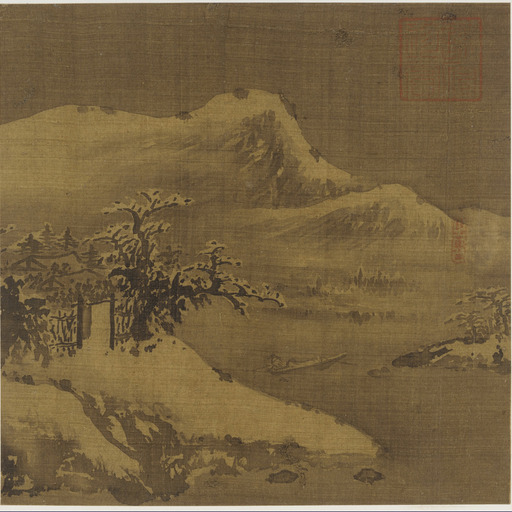
\includegraphics[width=0.2\textwidth, frame]{figures/diffusion/dataset_complete/Painting (4).jpg}}
    \quad
    \subfigure{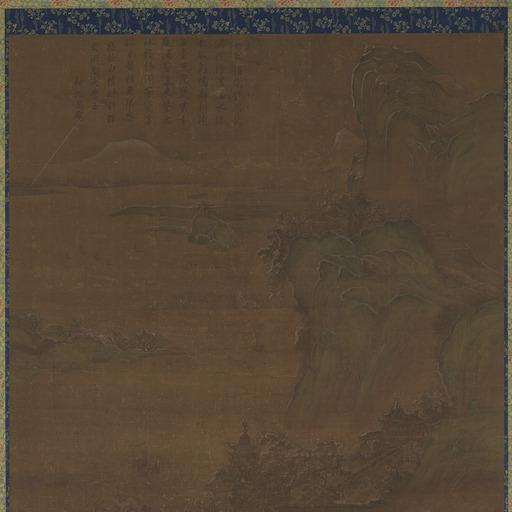
\includegraphics[width=0.2\textwidth, frame]{figures/diffusion/dataset_complete/Painting (5).jpg}}
    \subfigure{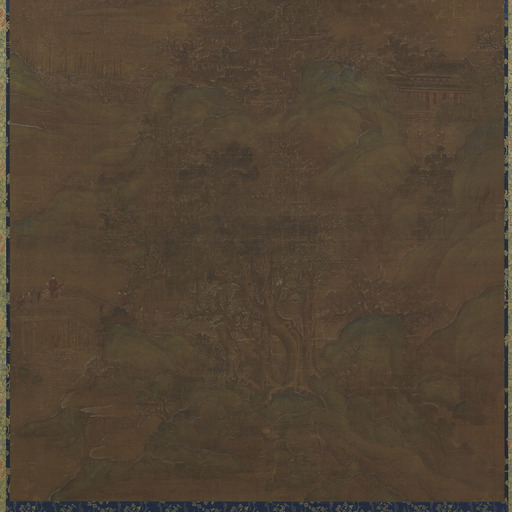
\includegraphics[width=0.2\textwidth, frame]{figures/diffusion/dataset_complete/Painting (6).jpg}}
    \subfigure{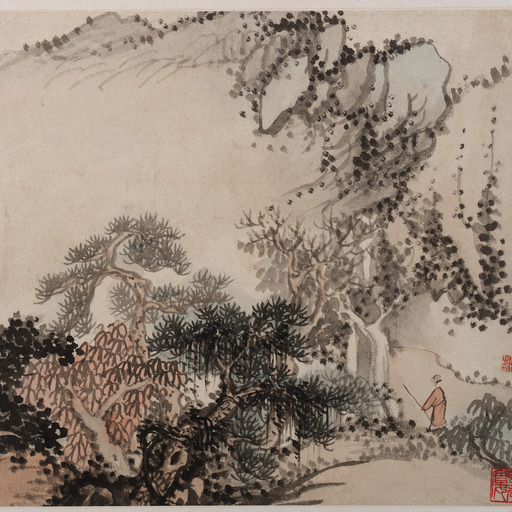
\includegraphics[width=0.2\textwidth, frame]{figures/diffusion/dataset_complete/Painting (7).jpg}}
    \subfigure{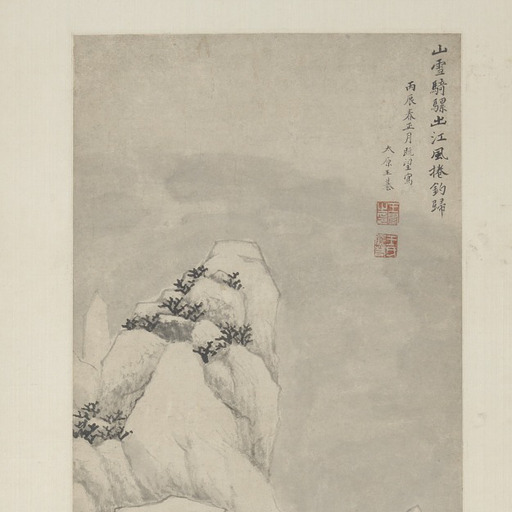
\includegraphics[width=0.2\textwidth, frame]{figures/diffusion/dataset_complete/Painting (8).jpg}}
    \caption{完整数据集中国画样本}\label{fig:complete_dataset_samples}
\end{figure}
\begin{figure}[ht]
    \centering
    \subfigure{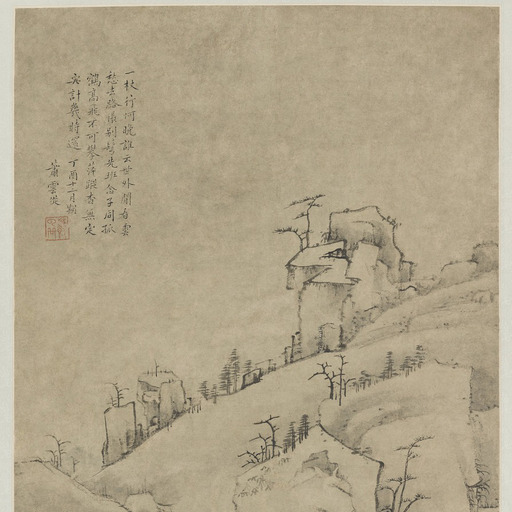
\includegraphics[width=0.2\textwidth, frame]{figures/diffusion/dataset_white/Painting (1).jpg}}
    \subfigure{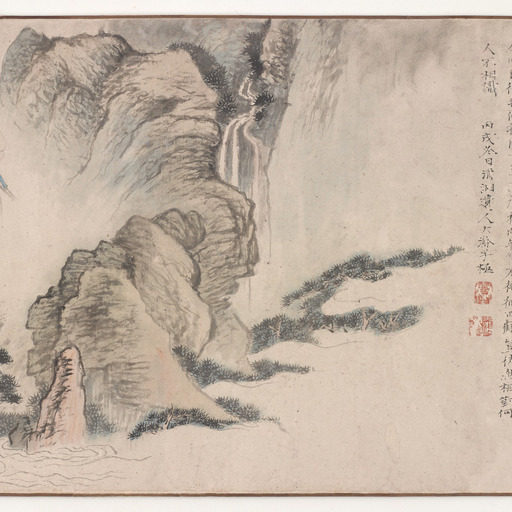
\includegraphics[width=0.2\textwidth, frame]{figures/diffusion/dataset_white/Painting (2).jpg}}
    \subfigure{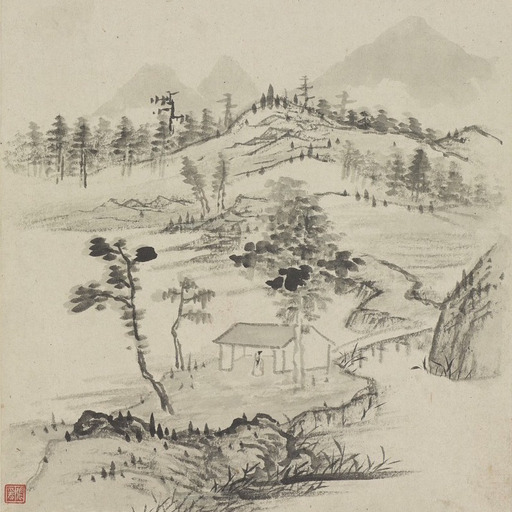
\includegraphics[width=0.2\textwidth, frame]{figures/diffusion/dataset_white/Painting (3).jpg}}
    \subfigure{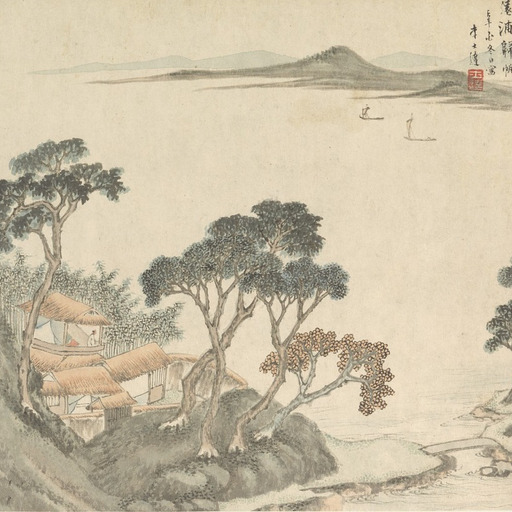
\includegraphics[width=0.2\textwidth, frame]{figures/diffusion/dataset_white/Painting (4).jpg}}
    \quad
    \subfigure{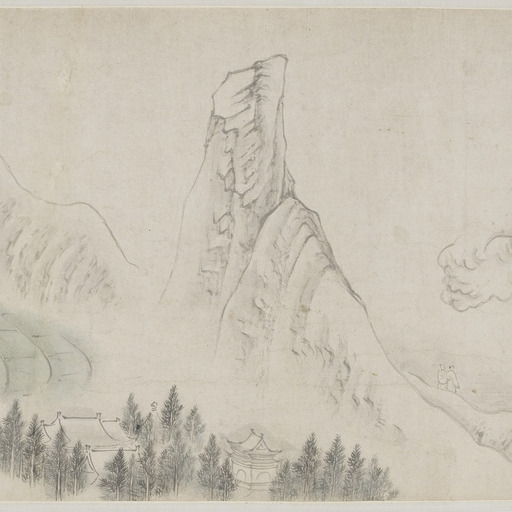
\includegraphics[width=0.2\textwidth, frame]{figures/diffusion/dataset_white/Painting (5).jpg}}
    \subfigure{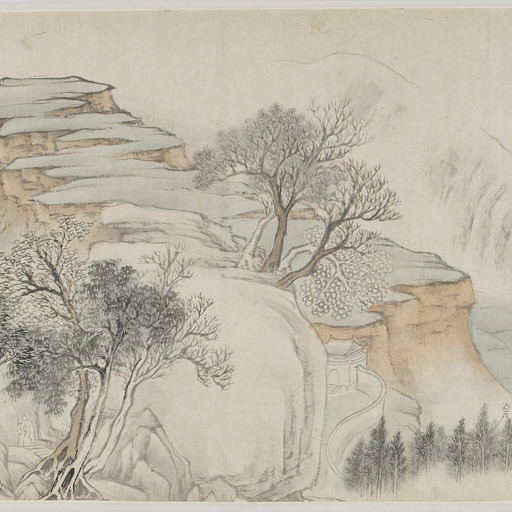
\includegraphics[width=0.2\textwidth, frame]{figures/diffusion/dataset_white/Painting (6).jpg}}
    \subfigure{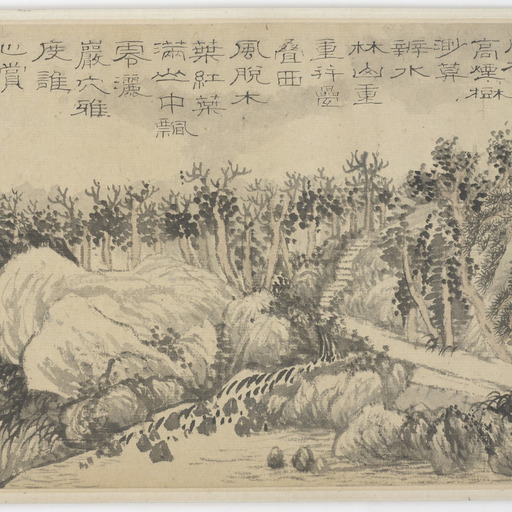
\includegraphics[width=0.2\textwidth, frame]{figures/diffusion/dataset_white/Painting (7).jpg}}
    \subfigure{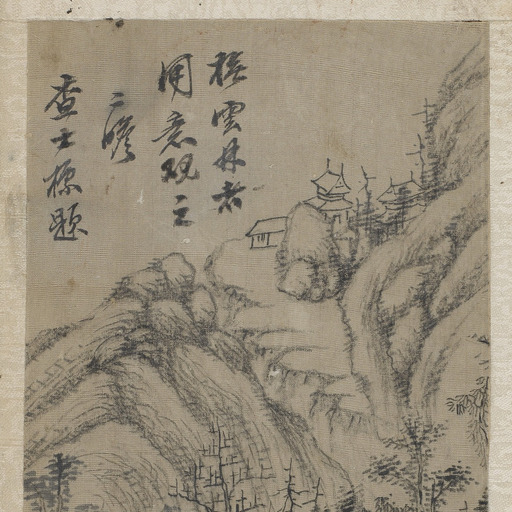
\includegraphics[width=0.2\textwidth, frame]{figures/diffusion/dataset_white/Painting (8).jpg}}
    \caption{浅色中国画数据集样本}\label{fig:white_dataset_samples}
\end{figure}
\begin{figure}[ht]
    \centering
    \subfigure{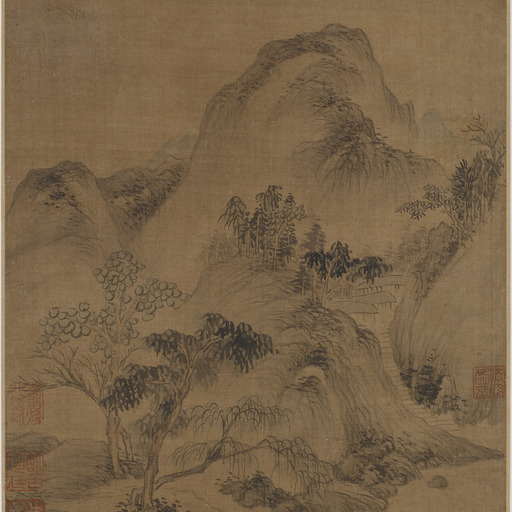
\includegraphics[width=0.2\textwidth, frame]{figures/diffusion/dataset_yellow/Painting (1).jpg}}
    \subfigure{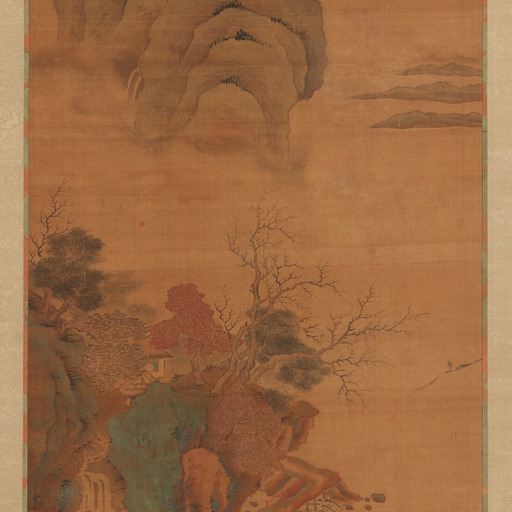
\includegraphics[width=0.2\textwidth, frame]{figures/diffusion/dataset_yellow/Painting (2).jpg}}
    \subfigure{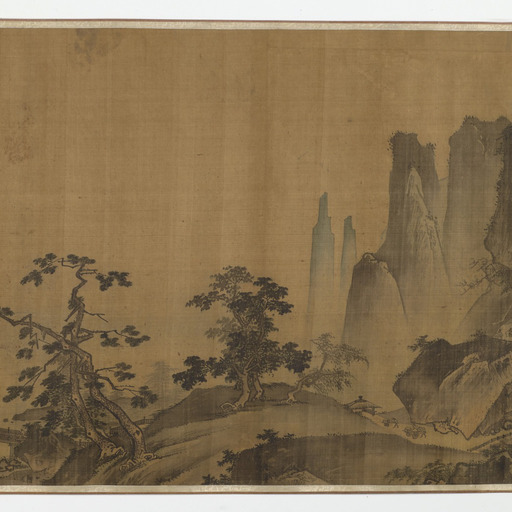
\includegraphics[width=0.2\textwidth, frame]{figures/diffusion/dataset_yellow/Painting (3).jpg}}
    \subfigure{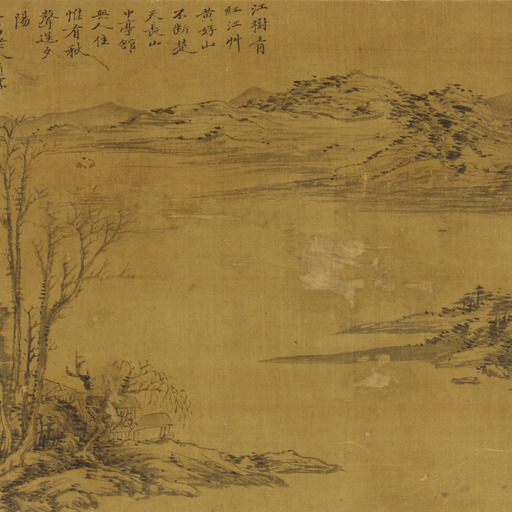
\includegraphics[width=0.2\textwidth, frame]{figures/diffusion/dataset_yellow/Painting (4).jpg}}
    \quad
    \subfigure{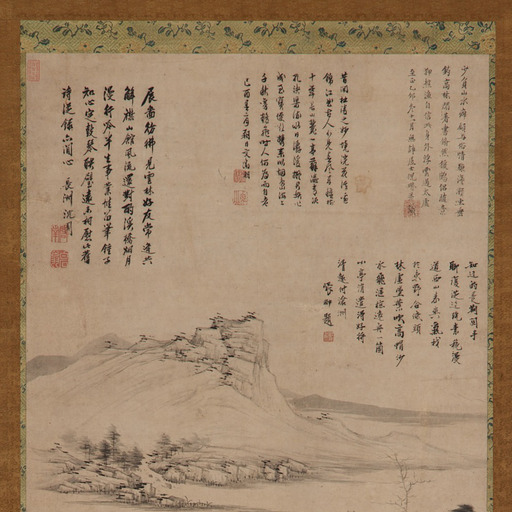
\includegraphics[width=0.2\textwidth, frame]{figures/diffusion/dataset_yellow/Painting (5).jpg}}
    \subfigure{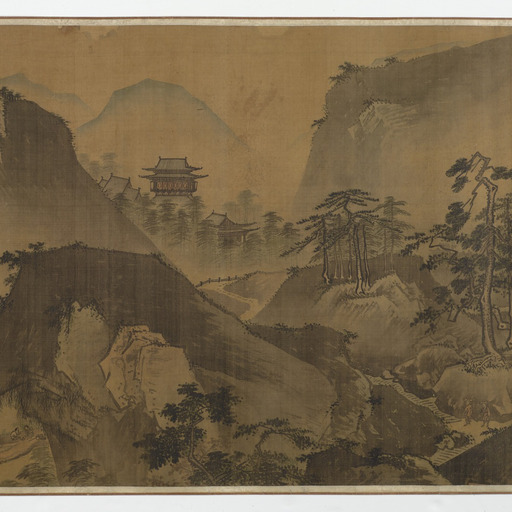
\includegraphics[width=0.2\textwidth, frame]{figures/diffusion/dataset_yellow/Painting (6).jpg}}
    \subfigure{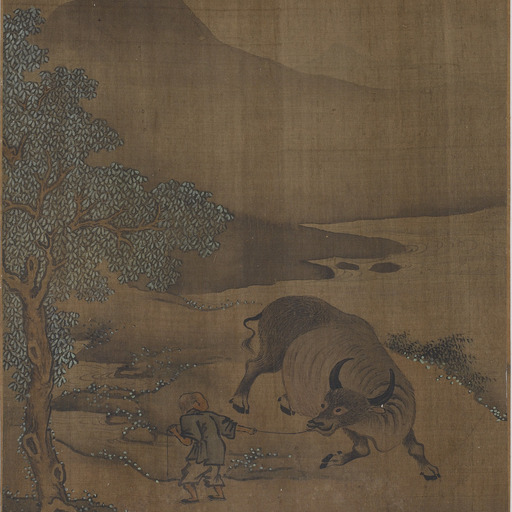
\includegraphics[width=0.2\textwidth, frame]{figures/diffusion/dataset_yellow/Painting (7).jpg}}
    \subfigure{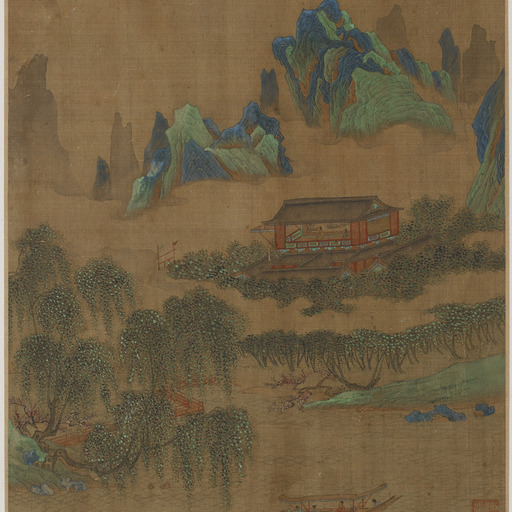
\includegraphics[width=0.2\textwidth, frame]{figures/diffusion/dataset_yellow/Painting (8).jpg}}
    \caption{深色中国画数据集样本}\label{fig:yellow_dataset_samples}
\end{figure}


\section{实验}

分别使用完整数据集、浅色中国画数据集、深色中国画数据集进行训练,
以生成高质量中国画,其中使用浅色中国画数据集依次进行了大批量和小批量训练。

各实验根据实际情况不同,使用不同GPU型号,不同实验共同的环境配置如下:
\begin{itemize}
    \item 操作系统:Ubuntu 20.04
    \item Python 编译器器:Python 3.8
    \item Pytorch 框架:1.12
    \item CUDA 版本:11.3
    \item 编辑器:Visual Studio Code 
\end{itemize}

不同实验扩散模型相同参数设置如下:
\begin{itemize}
    \item 图像大小:128*128
    \item 扩散步骤:1000步
    \item 采样步骤:250步
    \item 损失函数类型:L1距离
    \item 学习率:{$1\times10^{-5}$}
    \item 梯度累计步骤:2
\end{itemize}

\clearpage
\subsection{实验1-完整数据集生成中国画}

\begin{figure}[H]
    \centering
    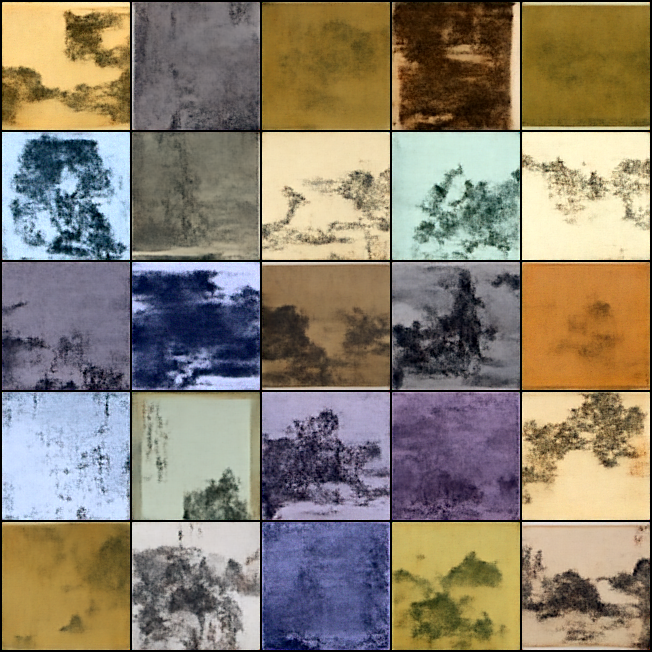
\includegraphics[width=0.8\textwidth]{figures/diffusion/results1/sample-16}
    \caption{实验1-完整数据集生成中国画采样图}\label{fig:diffusion_results1_sample16}
\end{figure}

\subsubsection{实验配置}
使用完整数据集,
在A100- 80GB GPU上,
以128为训练批量训练约15小时。
\subsubsection{实验结果与分析}

实验一结果如图{\ref{fig:diffusion_results1_sample16}}所示。
为减小比对模型不同训练阶段图像生成质量的误差,
采样20次,共获取20张图片并合并显示。
由于完整数据集中图片颜色丰富,
模型需要同时学习不同颜色深度中国画,
在计算资源有限情况下模型收敛需要更长时间,
此外,不同深度中国画混合训练容易造成中国画颜色混合,
降低图片生成质量,
为加快模型收敛与提高图片生成质量,
使用浅色中国画数据集和深色中国画数据集分别训练。

\subsection{实验2-浅色中国画数据集大批量训练}

\begin{figure}[H]
    \centering
    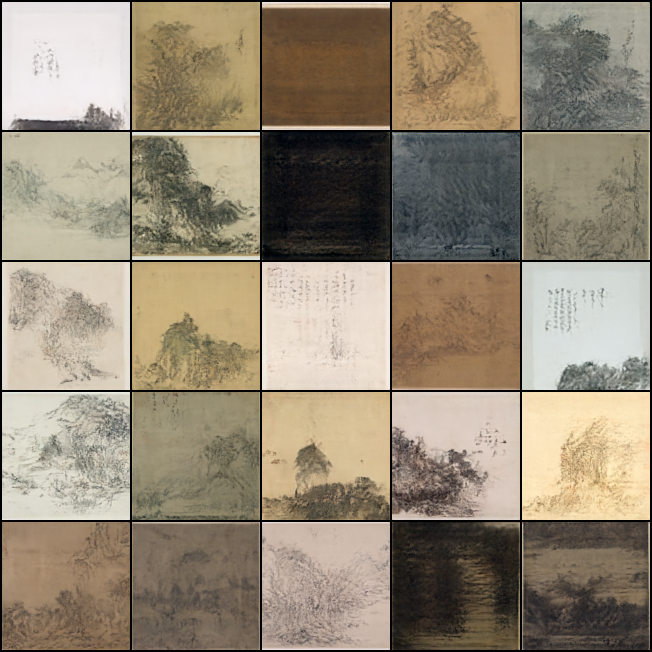
\includegraphics[width=0.8\textwidth]{figures/diffusion/results2/sample-70.png}
    \caption{实验2-浅色中国画数据集大批量训练生成中国画采样图}\label{fig:diffusion_results2_sample70}
\end{figure}

\subsubsection{实验配置}
使用浅色中国画数据集,
在A100- 40GB GPU上,
以64为训练批量,
训练约48小时。
\subsubsection{实验结果与分析}

图{\ref{fig:diffusion_results2_sample70}}为训练70轮后的采样图像,
相比于实验1使用完整数据集所生成的图像,
大部分图像颜色较浅,图像质量明显提升。
第四行{\footnote{以图像表格上方为第一行,左侧为第一列,坐标表示为(行,列)}}图像取得了与中国画非常相似的效果,
一些图像如{$(3,3),(3,5)$},已经可以生成与中国画中的落款相似的文字符号。
同时有一些图像如{$(2,3),(5,4)$},未成功生成中国画,
增大数据集容量、或使用数据增强技术,有望改善扩散模型无法将隐变量噪声空间映射到中国画空间的情况。






\subsection{实验3-浅色中国画数据集小批量训练}

\begin{figure}[H]
    \centering
    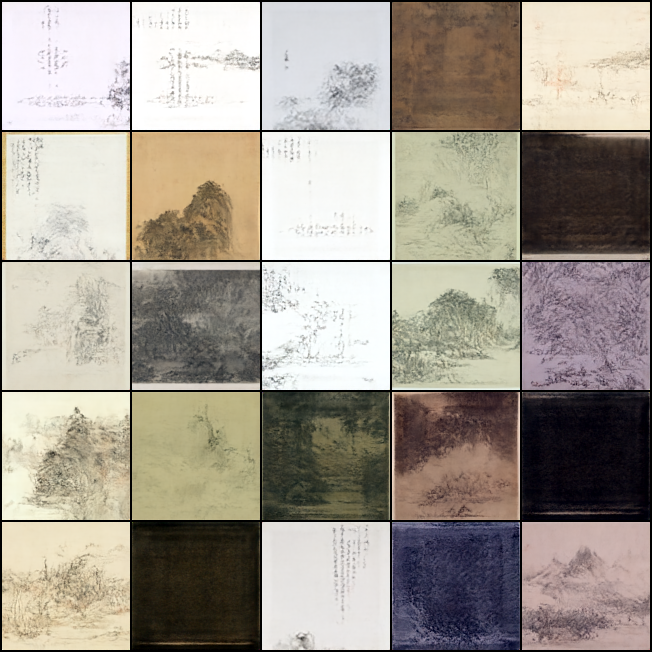
\includegraphics[width=0.8\textwidth]{figures/diffusion/results3/sample-80.png}
    \caption{实验3-浅色中国画数据集小批量训练生成中国画采样图}\label{fig:diffusion_results3_sample80}
\end{figure}

\subsubsection{实验配置}
使用浅色中国画数据集,
在3090- 24GB GPU上,
以32为训练批量训练约48小时。
\subsubsection{实验结果与分析}
图{\ref{fig:diffusion_results3_sample80}}为训练80轮后的采样图像,
相比于实验2,实验三仅仅改变了训练批量,
但产生了更多的无法成功生成中国画的情况,
如子图{$(2,5),(4,2),(4,5),(5,2),(5,4)$}生成颜色过深图像,
子图{$(1,1),(1,2),(1,5),(2,3),(3,3)$}生成颜色过浅图像。
对比实验2与实验3可得,更大的训练批量有助于生成更高质量的中国画。





\subsection{实验4-深色中国画数据集生成中国画}

\begin{figure}[H]
    \centering
    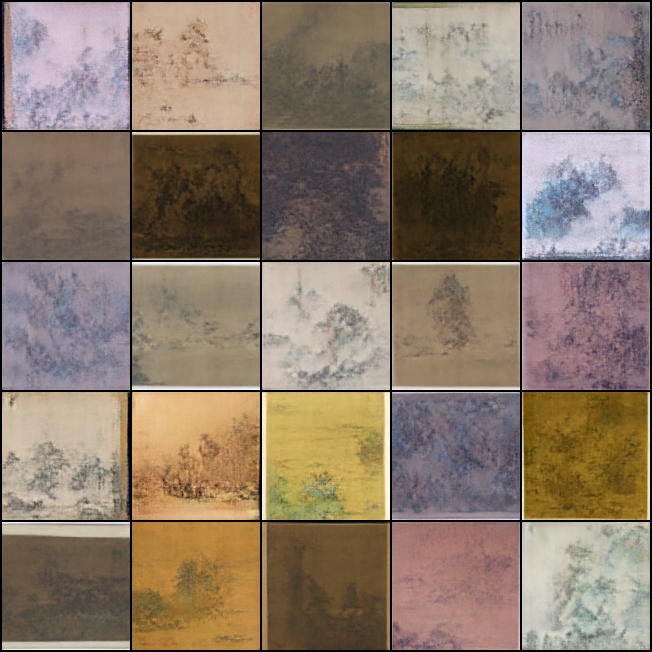
\includegraphics[width=0.8\textwidth]{figures/diffusion/results4/sample-33}
    \caption{实验4-深色中国画数据集生成中国画采样图}\label{fig:diffusion_results4_sample33}
\end{figure}

\subsubsection{实验配置}
使用深色中国画数据集,
在A100- 40GB GPU上,
以64为训练批量训练约36小时。
\subsubsection{实验结果与分析}


图{\ref{fig:diffusion_results4_sample33}}为训练33轮后的采样图像。
实验4与实验2类似,训练批量都为64,都在A100- 40GB GPU上训练。
不同的是,实验4使用深色中国画数据集,而实验2使用浅色中国画数据集。
实验4相对于实验1,得到的图像与中国画更相似;
相比于实验2,生成的中国画的颜色更加丰富。
